\scanpage{11}
Il faut prouver qu'on a bien un foncteur.

a) $\varphi_{X,X}(\operatorname{id}_X)=\Delta_X$. En effet,
\deleted{\unsure{ce qui est la définition}}\inserted{c'est la définition} de $\Delta_X$!

b) \diagram{\begin{tikzcd}X\arrow[r,no head,"f"]&Y\arrow[r,no head,"g"]&Z\end{tikzcd}}
\[
\varphi(g)\varphi(f)=\varphi(gf)
\]
Le premier mb est
\[
p_{31*}\left(\underbrace{p_{32}^*(\varphi(g))}_{\substack{p_{32}^*(\Gamma_{g*}(1))\\=\deleted{\unsure{\mu_*}}\lambda_*(\mu^*(1))=\lambda_*(1)}}\;
\underbrace{p_{21}^*(\varphi(f))}_{\substack{p_{21}^*\Gamma_{f*}(1)\\=\lambda'_*(\mu'^*(1))=\lambda'_*(1)}}\right)
\]
\diagram{\begin{tikzcd}[column sep=small,row sep=large]
&X\times Z\arrow[dl,"\mu'"']\arrow[dr,"\lambda'"]&&X\times Y\arrow[dl,"\lambda=\operatorname{id}_X\times\Gamma_g"']\arrow[dr,"\mu"]&\\
X\arrow[dr,"\Gamma_f"']&&X\times Y\times Z\arrow[dl,"p_{21}"]\arrow[d,"p_{31}"]\arrow[dr,"p_{32}"']&&Y\arrow[dl,"\Gamma_g"]\\
&X\times Y&X\times Z&Y\times Z&
\end{tikzcd}}
\[
\varphi(g)\varphi(f)=p_{31*}(\unsure{\lambda^*_*|\lambda_*}(1)\,\lambda'_*(1))
\]
Mais
\[
\lambda_*(1)\lambda'_*(1)=\lambda_*\left(\underbrace{\lambda^*(\lambda'_*(1))}_{\Gamma_{f*}(\Gamma_{gf}^*(1))=\Gamma_{f*}(1)}\right)
\qquad\fbox{\text{(form. proj)}}
\]
\diagram{\begin{tikzcd}[column sep=small,row sep=large]
&&X\arrow[dl,"\Gamma_{gf}"']\arrow[dr,"\Gamma_f"]&&\\
&X\times Z\arrow[dl,"\mu'=p_X"']\arrow[dr,"\lambda'=\unsure{\Gamma_f}\times Z"]&\text{(cartésien)}&X\times Y\arrow[dl,"\lambda=\operatorname{id}_X\times\Gamma_g"']\arrow[dr,"\mu=p_Y"]&\\
X\arrow[dr,"\Gamma_f"']&&X\times Y\times Z\arrow[dl,"p_{21}"]\arrow[d,"p_{31}"]\arrow[dr,"p_{32}"']&&Y\arrow[dl,"\Gamma_g"]\\
&X\times Y&X\times Z&Y\times Z&
\end{tikzcd}}
\[
=\lambda_*\Gamma_{f*}(1)=\nu_*(1)
\]
où $\nu:X-X\times Y\times Z$ est donné
par $\nu(x)=(x,f(x),gf(x))$.
\diagram{\begin{tikzcd}[column sep=small,row sep=small]
x\arrow[r,mapsto]&(x,gf(x))&(x,f(x),gf(x))\arrow[l,mapsto]\\
x\arrow[r,no head]&(x,f(x))\arrow[r,mapsto]&(x,f(x),gf(x))
\end{tikzcd}}
\margin{\deleted{\unsure{f(x)}} $(x,f(x),z)$\quad $(x,y,g(y))$\quad $(x,f(x),gf(x))$}
D'où
\[
\varphi(g)\varphi(f)=p_{31*}(\nu_*(1))=\Gamma_{gf*}(1)=\varphi(gf)\qquad\mathrm{OK}.
\]

\figure{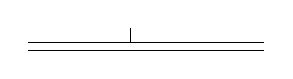
\begin{tikzpicture}\draw (0,0)--(3,0);\draw (0,-.10)--(3,-.10);\draw (1.3,0)--(1.3,.18);\end{tikzpicture}}

Définissons le foncteur $\psi$, \inserted{avec $\psi(X)=A(X)$,} i.e. pour
$u\in\operatorname{Hom}_{\mathcal V^A}(X,Y)=A(X\times Y)$, et $x\in A(X)$, définissons $u(x)\in A(Y)$
par formule \deleted{\unsure{u(x)}}
\[
u(x)=p_{2*}(u\,p_1^*(\unsure{x|u}))
\]
Prouvons que l'on a bien une \uline{loi fonctorielle}.
\mspage{10}
